\documentclass[12pt,a4paper]{article}
\linespread{1.0}
% Language setting
% Replace `english' with e.g. `spanish' to change the document language
\usepackage[english]{babel}
\usepackage[colorlinks,linkcolor=blue]{hyperref}
% Set page size and margins
% Replace `letterpaper' with `a4paper' for UK/EU standard size
\usepackage[letterpaper,top=2cm,bottom=2cm,left=3cm,right=3cm,marginparwidth=1.75cm]{geometry}
\usepackage{indentfirst}
\usepackage[T1]{fontenc}
\usepackage[utf8]{inputenc}
\usepackage{authblk}
% Useful packages
\usepackage{amsmath}
\usepackage{amsfonts,amssymb}
\usepackage{graphicx}
\usepackage[colorlinks, linkcolor = blue]{hyperref}
% \usepackage{indentfirst} 
\usepackage{float}
\setlength{\parindent}{2em}
\title{Insurance charge estimation based on regression analysis}

\author[1]{Dake Li}
\author[2]{Likun Lin}
\affil[1]{Department of Mathematics, Fudan University}
\affil[2]{Department of Mathematics, City University of Hong Kong}
\begin{document}
\maketitle

\begin{abstract}
In this article, we selected a set of data from Kaggle website about medical insurance charge, provided with BMI, age, whether smoking or not. By analysing this dataset, we aimed to predict the corresponding insurance charges for new BMI-age-smoking data. We mainly set up a linear regression model. However, in this process, we found that there was a significant difference between the data respect to smokers and non-smokers in the sample. Therefore, we classified the smokers and non-smokers into two categories and established prediction models separately.
\end{abstract}

\indent
\section{Motivation and Background}
The role of medical insurance in society is multifaceted. In terms of individuals, we want to build up a suitable expectation of the expenses on ourselves' medical insurance. Therefore, given personal information, a prediction model of the insurance charge is very useful. As taught in this course, linear regression model is a very powerful tool for people to estimate the relation between two variables. Since every function has a best linear approximation with its first-order derivatives in a neighbourhood, linear regression is especially useful to model some relations locally. In this article, we mainly built up a linear regression model to predict one's medical insurance charge in the future, based on his or her BMI, age, and whether smoking or not.

\section{Objectives}
The main objective of this article is to set up a prediction model of medical insurance charges, based on one's BMI, age, and whether smoking.

\section{Data Collections and Data Preprocessing}
\subsection{Data Collection}
We fetch the dataset from the website Kaggle (Data source: \url{https://www.kaggle.com/datasets/mirichoi0218/insurance}). This dataset contains a bunch of samples of the medical insurance charges, together with the customers' personal information. The original data has too many features, such as the customer's sex, region, have children yet or not and so on, but in order to have clearer insights, we want to take only a few features into consideration. 
\begin{figure}[H]
\centering
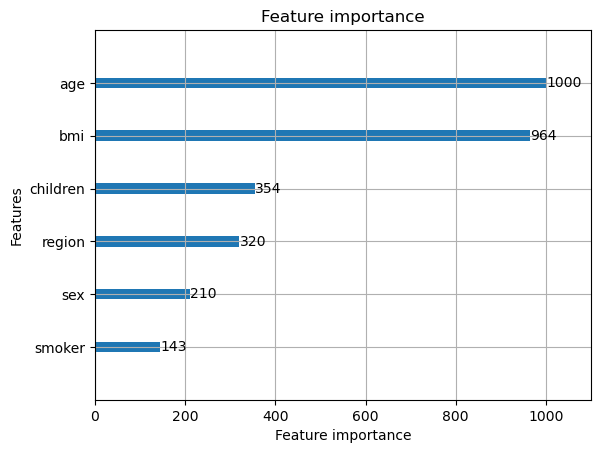
\includegraphics[width = 0.6\textwidth]{feature_importance.png}
\caption{Feature Importance (given by xgboost)}
\end{figure}
\par By XGBoost analysis, we conclude that the most improtant two features are age and BMI. In addition, from our life experience, whether smoking or not is also non-negligible.  Therefore, we still label our selected data with "smoker" or "non-smoker".
\begin{figure}[H]
\begin{minipage}[t]{0.48\textwidth}
\centering
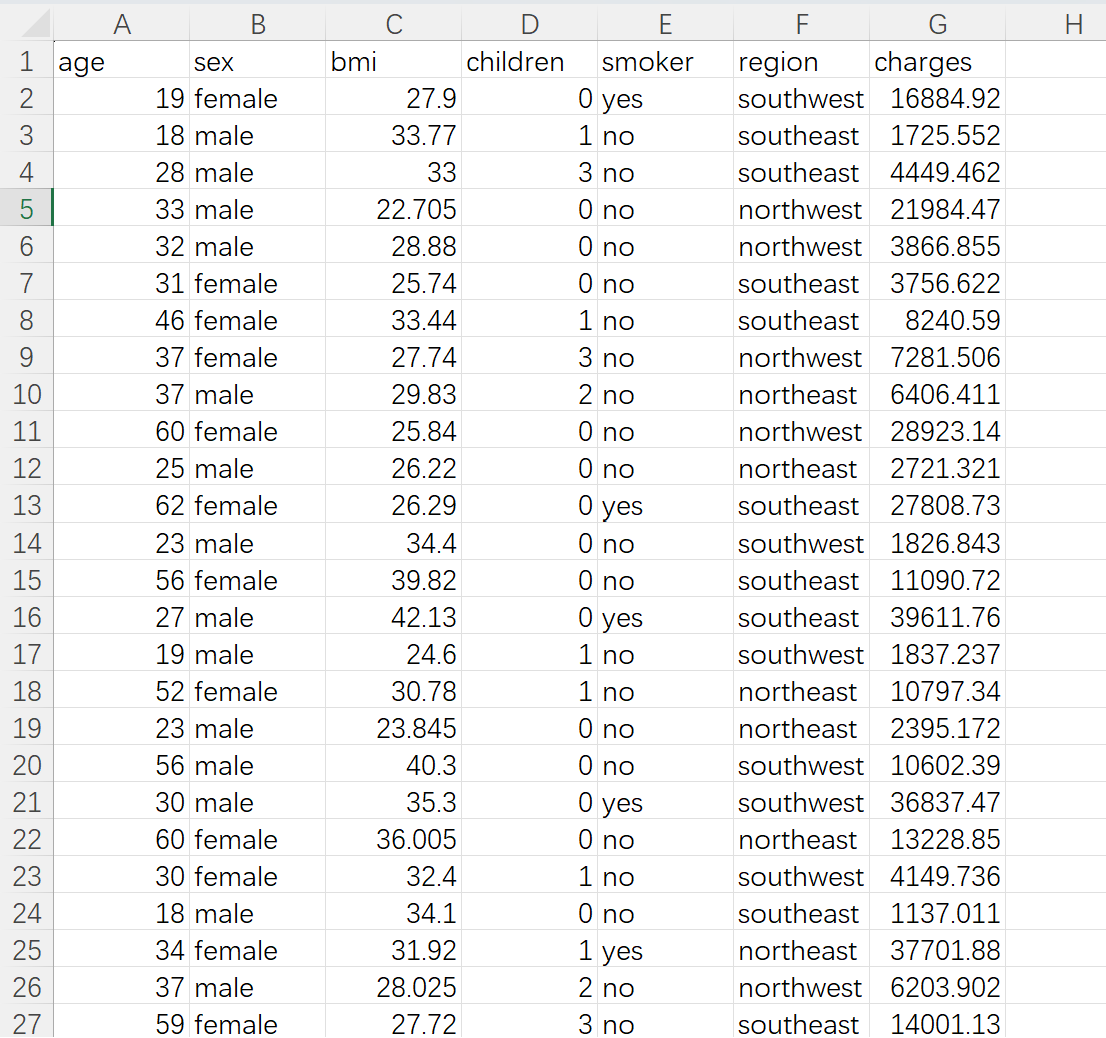
\includegraphics[width = 0.8\textwidth]{original_data.png}
\caption{Part of Original Data}
\end{minipage}
\begin{minipage}[t]{0.48\textwidth}
\centering
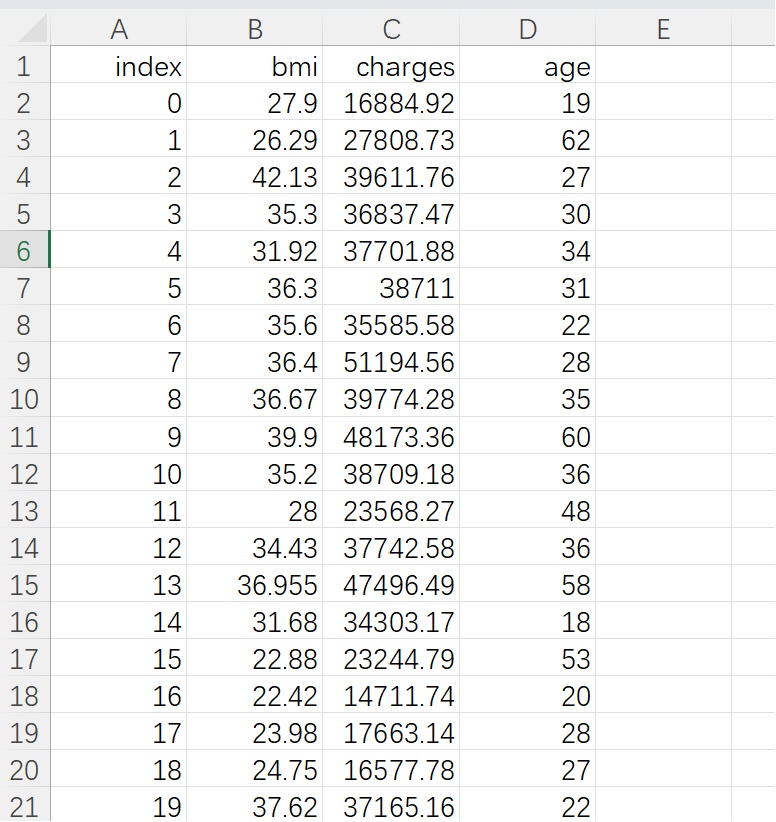
\includegraphics[width = 0.7\textwidth]{selected_data.png}
\caption{Part of Selected Data}
\end{minipage}
\end{figure}
 
\subsection{Data Preprocessing}
Firstly, it is observed that the data label of 'smoker' and 'non-smoker' led to a significant gap in the insurance charge, just as figure 1 and figure 2 show. 

\begin{figure}[H]
\centering
\begin{minipage}[t]{0.48\textwidth}
\centering
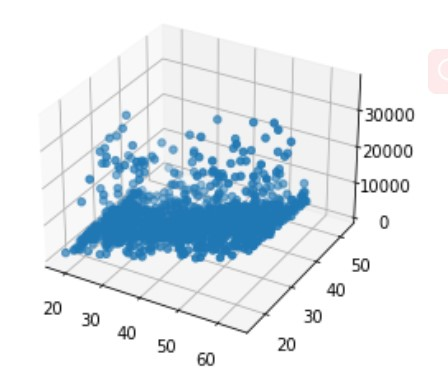
\includegraphics[width=6cm]{nonsmokeroverall.jpg}
\caption{Nonsmoker's condition}
\end{minipage}
\begin{minipage}[t]{0.48\textwidth}
\centering
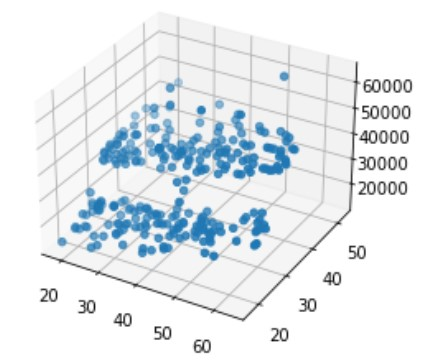
\includegraphics[width=6cm]{smokeroverall.jpg}
\caption{Smoker's condition}
\end{minipage}
\end{figure}

According to this observation, we intend to develop different prediction models for each of the condition. 
\par For each category(smoker or non-smoker), we randomly separate the raw data into two parts, that is, 70\% of the raw data to be the training set, and the remaining 30\% to be the test set.

\section{Clustering and Classification}
\subsection{Smokers' condition}
Firstly, we begin with the category of smokers.\par 
By observation of the BMI-charge(figure 3) and the age-charge(figure 4) figure, it is reasonable to believe that the category of smokers can be also divided into two parts, where each part possesses different properties. 

\begin{figure}[H]
\centering
\begin{minipage}[t]{0.48\textwidth}
\centering
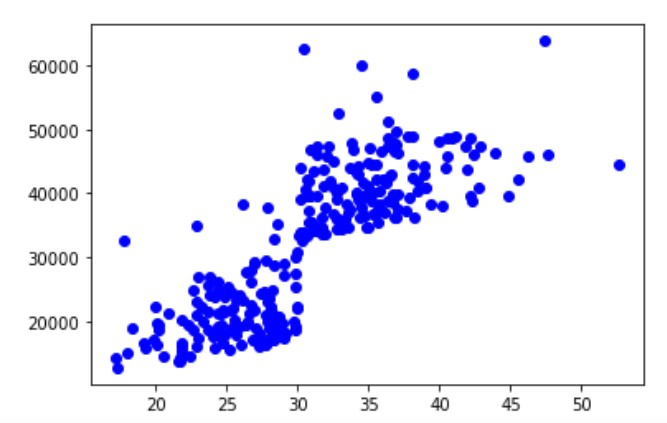
\includegraphics[width=6cm]{bmi-charge smoker.jpg}
\caption{BMI-charges figure}
\end{minipage}
\begin{minipage}[t]{0.48\textwidth}
\centering
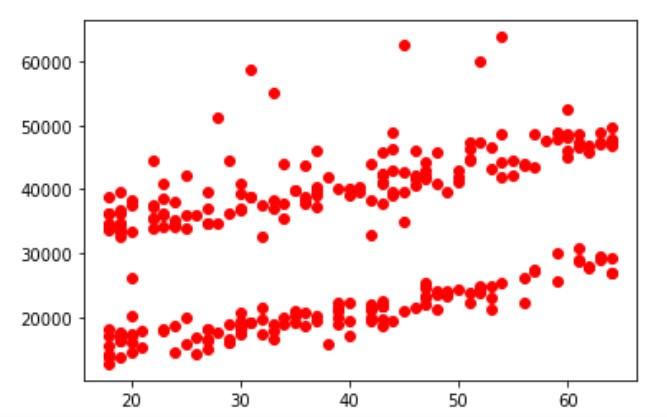
\includegraphics[width=6cm]{age-chargesmoker.jpg}
\caption{Age-charge figure}
\end{minipage}
\end{figure}

The following pair-plot figure provides more evidence that the dataset of smoker category has some intrinsic partition.

\begin{figure}[H]
\centering
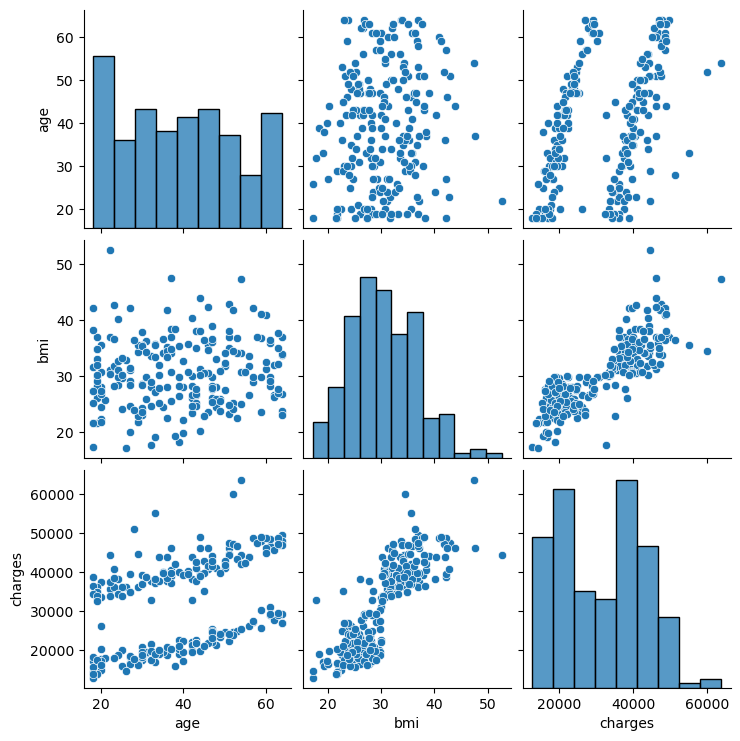
\includegraphics[width = 0.7\textwidth]{pairplot.png}
\caption{Pair-plot: age, BMI, charges}
\end{figure}

\par We conclude that the category of smoker can be further divided into two parts. The next idea is to apply linear regression on each part one by one.
\par The specific steps are:
\begin{enumerate}
\item Do clustering on the training set(70\% of the whole smoker data). 
\item Label the clusters by "class 1" and "class 2".
\item Using the obtained label, train a SVM model to classify.
\item Do linear regression on the each cluster.
\item For test set, we use the trained SVM to assign the label and apply the linear regression.
\end{enumerate}

The following figures show the result of out clustering:
\begin{figure}[H]
\centering
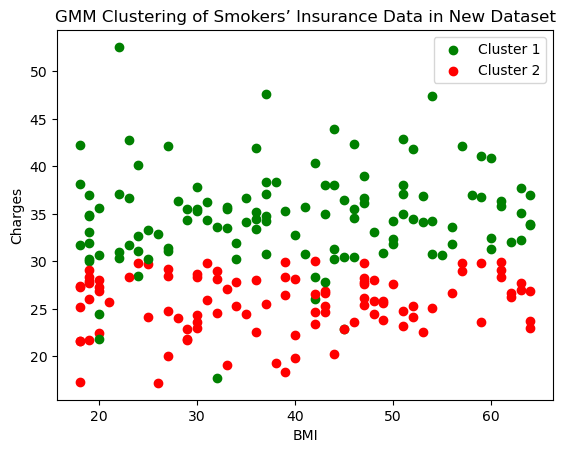
\includegraphics[width=0.6\textwidth]{GMM_clustering_smoker.png}
\caption{GMM Clustering of Smokers Category}
\end{figure}
\begin{figure}[H]
\centering
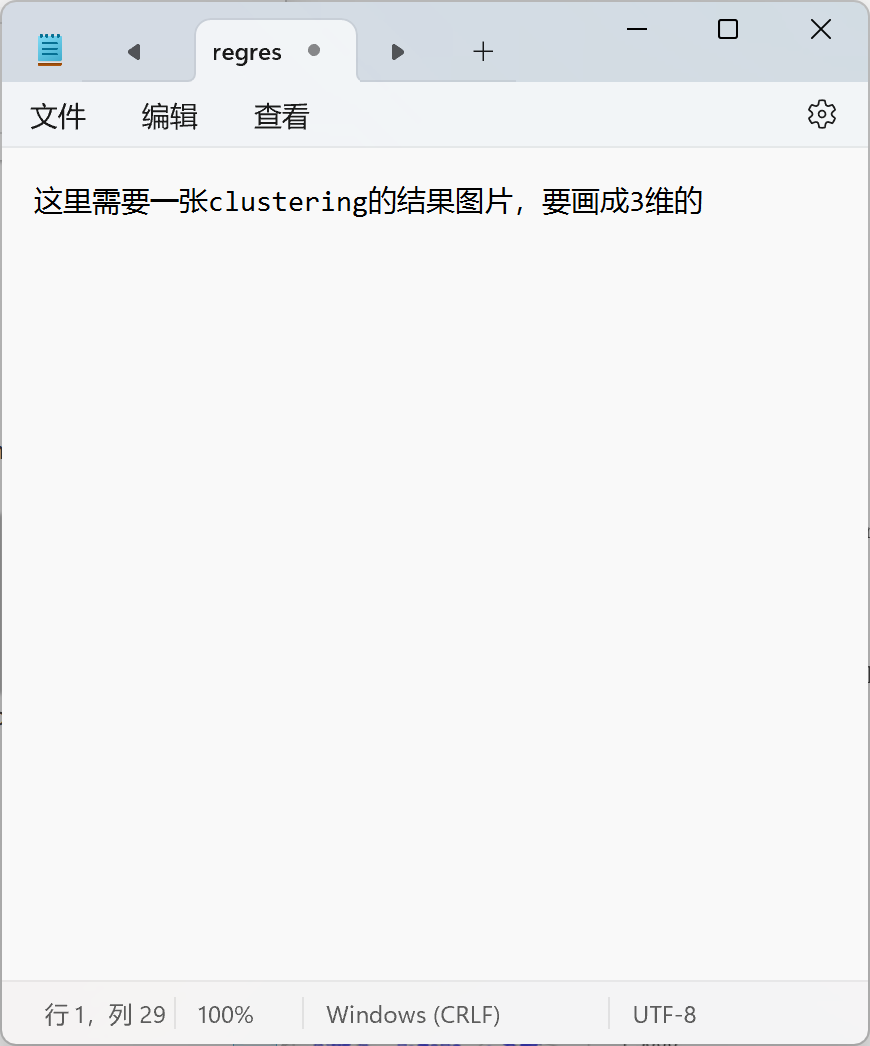
\includegraphics[width = 0.6\textwidth]{clustering_smoker_3d_plot.png}
\caption{3D plot for clustering result of smokers}
\end{figure}

According to the above analysis, the smoking population data can be divided into two clusters: high charge and low charge. 

\subsection{Non-smokers' condition}
By observation of the scatter plot, we can still find two clusters in the non-smoker data. 

\begin{figure}[H]
\centering
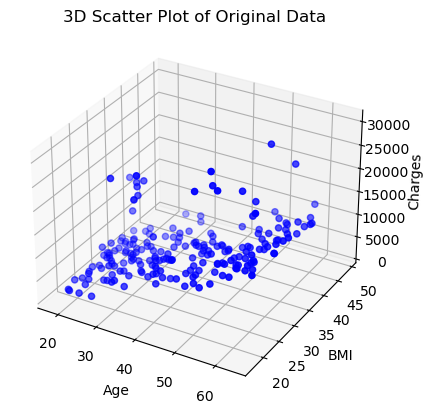
\includegraphics[width=0.6\textwidth]{non_smoker_scatter.png}
\end{figure}

We apply the same steps shown in the smokers' condition, 
\begin{figure}[H]
\centering
\begin{minipage}[t]{0.48\textwidth}
\centering
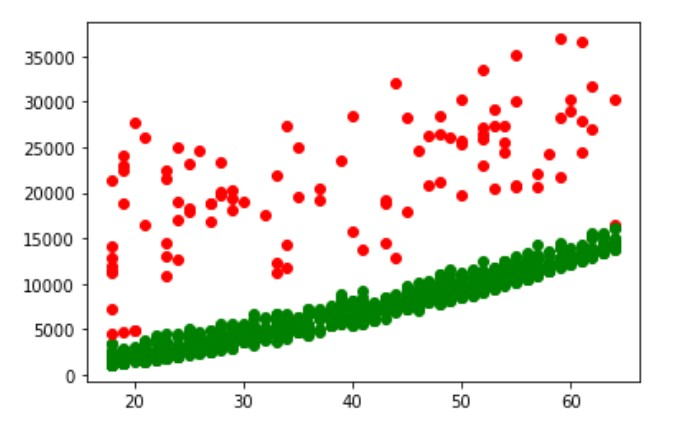
\includegraphics[width=6cm]{GMM RESULT with nonsmoker.jpg}
\caption{GMM result under nonsmoker condition}
\end{minipage}
\begin{minipage}[t]{0.48\textwidth}
\centering
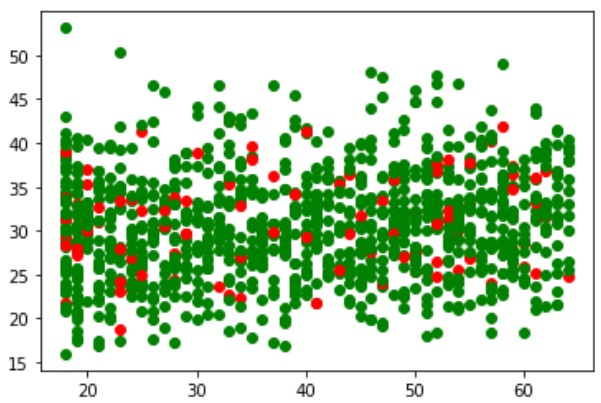
\includegraphics[width=6cm]{SVM2.jpg}
\caption{GMM cluster result on age bmi of non-smoker condition}
\end{minipage}
\end{figure}

\section{Ordinary Linear Regression model}
\newcommand{\x}{\mathbf{x}}
\newcommand{\y}{\mathbf{y}}
\newcommand{\w}{\mathbf{w}}
\newcommand{\norm}[1]{\left\Vert #1 \right\Vert}
We use the ordinary least squares method to do the linear regression. To be more specific, suppose $(x_1^i,x_2^i,y^i)\in \mathbb{R}^2 (i=1,2,\dots,N)$ are our data points, where $x_1^i$ denotes age, $x_2^i$ denotes BMI, and $y^i$ denotes charge. Our goal is to find a vector $\w = (b_0,b_1,b_2)\in \mathbb{R}^3$ such that $\w$ minimizes the loss function:
$$
L(\w) = \sum_{i=1}^{N}\left[ y^i - (b_0+b_1x_1^i+b_2x_2^i)\right]^2 = \norm{\y - X\w}_2^2
$$
where 
$$
\y = 
\begin{pmatrix}
y^1 \\ y^2 \\ \vdots \\y^N
\end{pmatrix}\in \mathbb{R}^N, \quad
X = 
\begin{pmatrix}
1 & x_!^1 & x_2^1 \\
1 & x_!^2 & x_2^2 \\
\vdots & \vdots & \vdots \\
1 & x_!^N & x_2^N \\
\end{pmatrix}\in \mathbb{R}^{N\times 3}.
$$
To minimize the loss function, we seek for stationary point. Let $\nabla L(\w)=0$ we get
$$ \w^{*} = (X^T X)^{-1}X^T \y.$$

The result of linear regression for smokers category:
\begin{figure}[H]
\begin{minipage}[t]{0.48\textwidth}
\centering
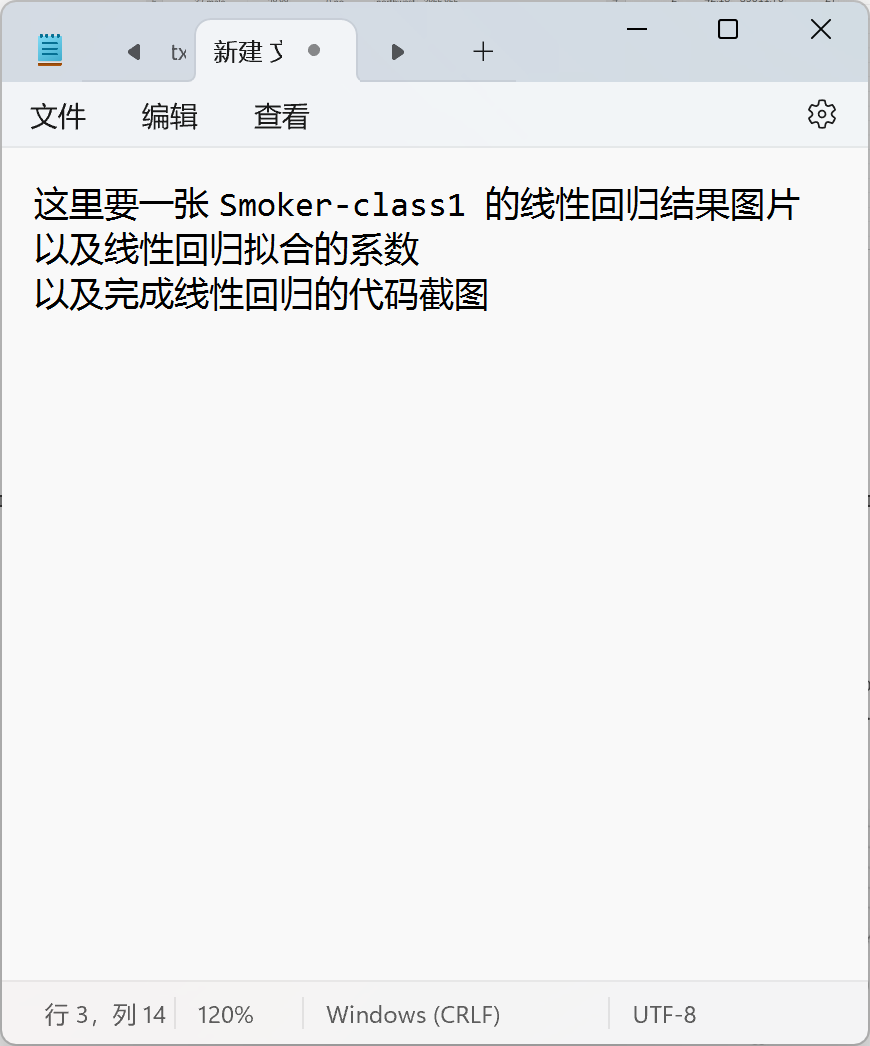
\includegraphics[width = 0.7\textwidth]{regression_smoker_class1.png}
\caption{Smoker:class 1}
\end{minipage}
\begin{minipage}[t]{0.48\textwidth}
\centering
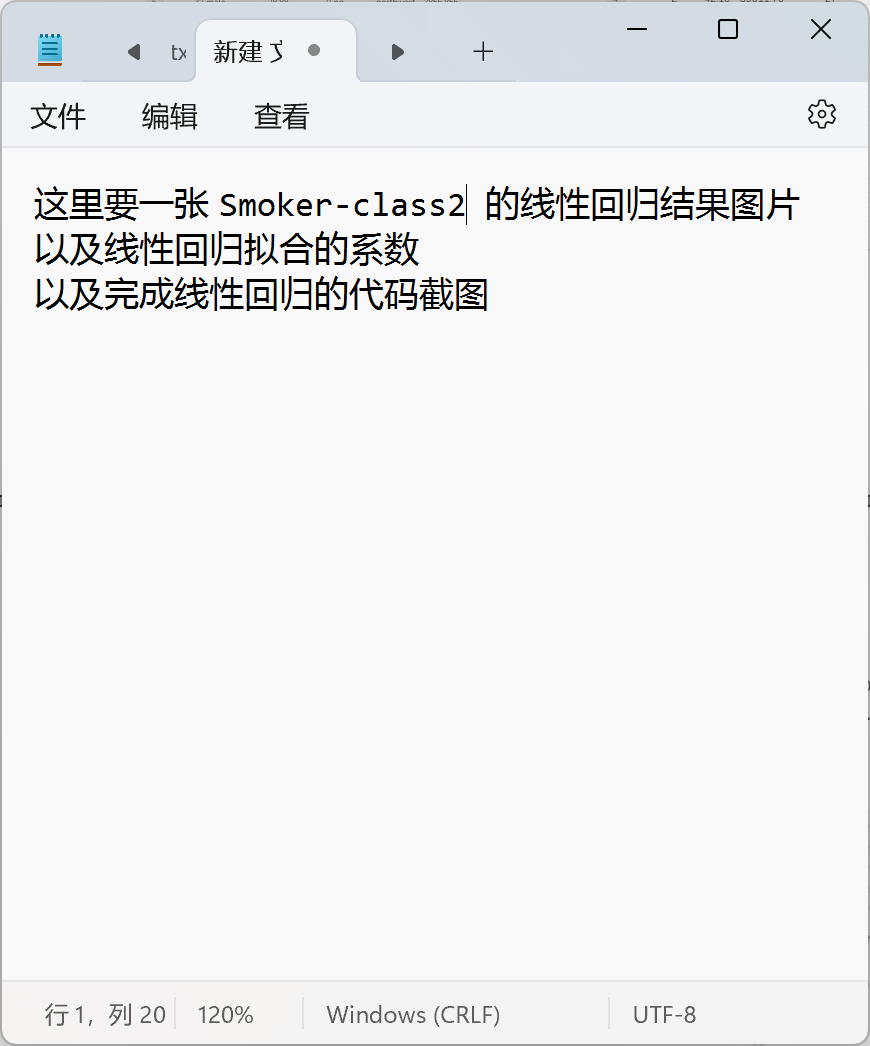
\includegraphics[width = 0.7\textwidth]{regression_smoker_class2.png}
\caption{Smoker:class2}
\end{minipage}
\end{figure}

The result of linear regression for non-smokers category:
\begin{figure}[H]
\begin{minipage}[t]{0.48\textwidth}
\centering
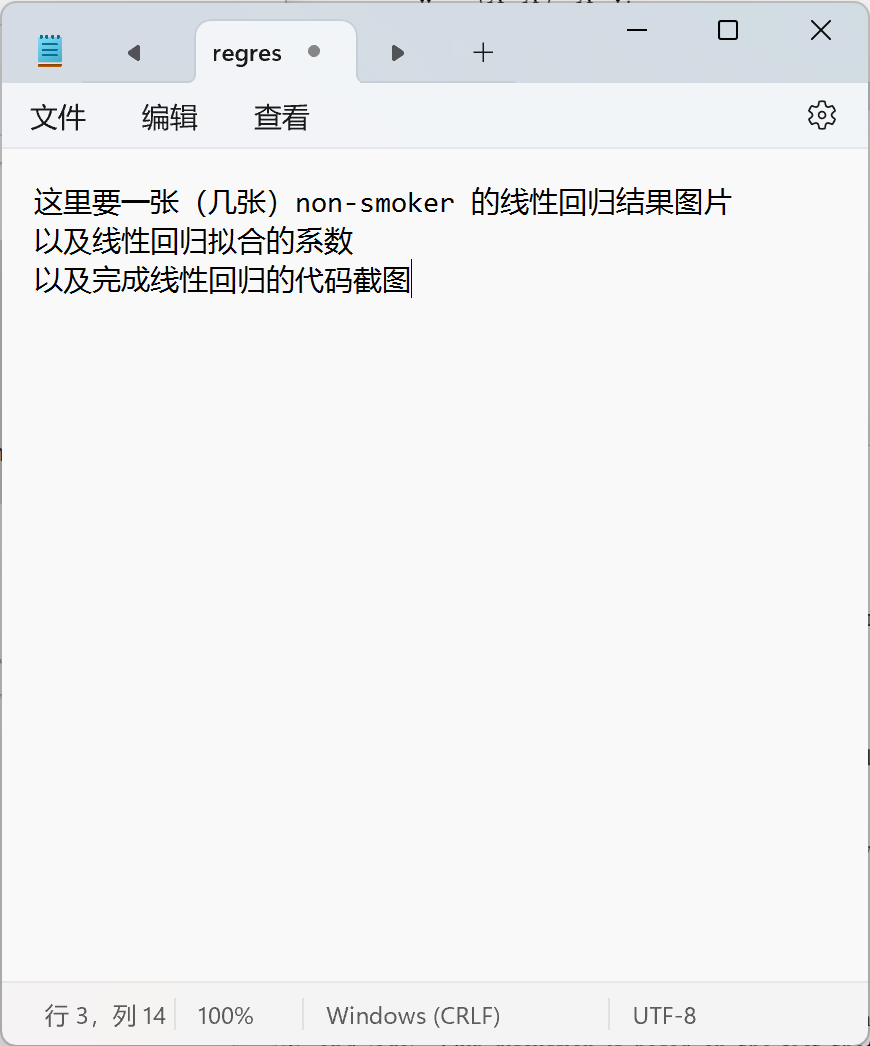
\includegraphics[width = 0.7\textwidth]{regression_non-smoker.png}
\caption{Non-smoker}
\end{minipage}
\begin{minipage}[t]{0.48\textwidth}
\centering
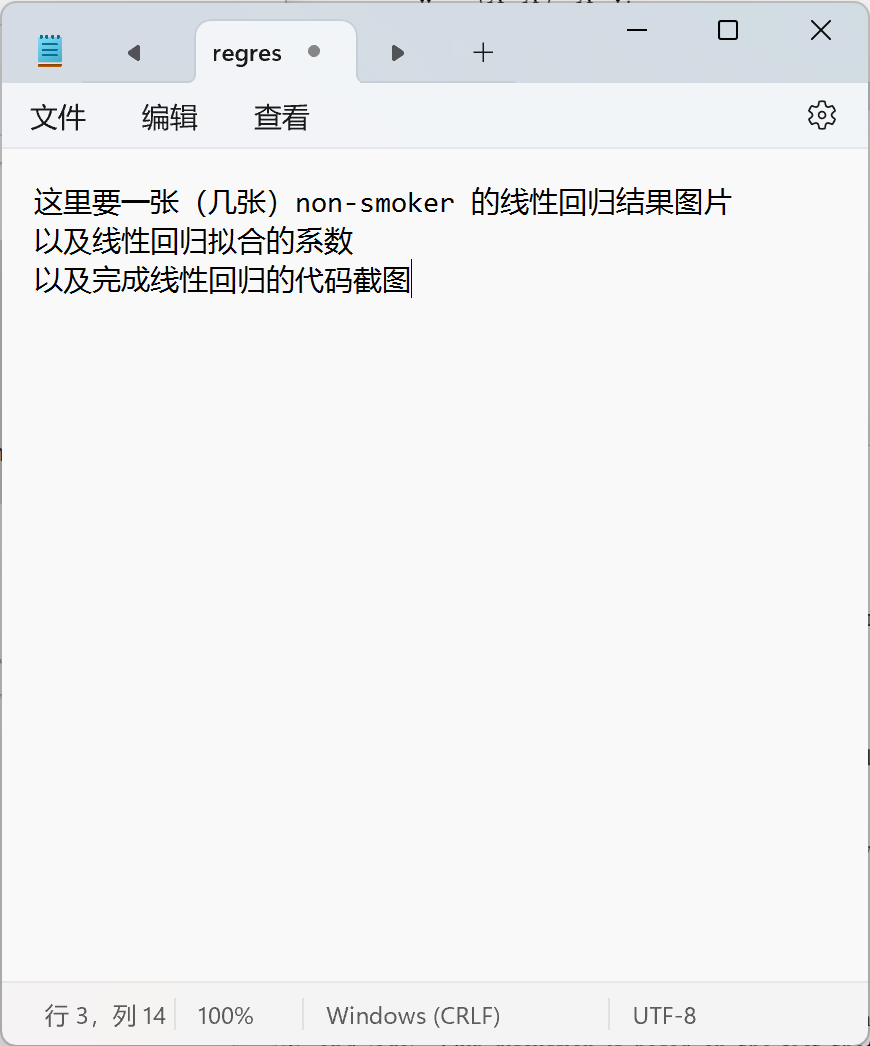
\includegraphics[width = 0.7\textwidth]{regression_non-smoker.png}
\caption{Non-smoker}
\end{minipage}
\end{figure}

%\subsection{Simple Linear Regression with non-smoker category}
%Consequently, Simple linear regression between age and charges is applied.
%For input feature age (represented as X), the estimator for charges (represented as $\widehat{y}(x)$) can be calculated as:
%$$\widehat{y}(x)=\widehat{\mu}_{Y \mid X=x}=\widehat{\beta}_{0}+\widehat{\beta}_{1} X $$,
%The simple linear regression model from the R code is $Y = -3298.954 + 267.753x$, and $R^{2}$ is 0.8536, which is shown in figure 13.
%Meanwhile, based on
%$$\widehat{y}(x) \sim N\left(\mu_{Y \mid X=x}, \sigma^{2}\left(\frac{1}{n}+\frac{|x-\bar{x}|^{2}}{s_{x x}}\right)\right)$$
%$$Y \mid(X=x)-\widehat{y}(x) \sim N\left(0, \sigma^{2}\left(1+\frac{1}{n}+\frac{|x-\bar{x}|^{2}}{s_{x x}}\right)\right)$$
%With the unbiased estimator $s$ for $\sigma$, the  $0.95 $ confidence interval and the prediction interval are calculated and shown in figure 14.
%
%\subsection{Multiple Linear Regression with higher-charges smokers category }
%Firstly, the training set is also cleaned by means of controlling the standardized residual between -2 and 2.
%Then, multiple linear regression is applied with the input features such as BMI and age, whose result is shown in figure 15. From the result, it is obvious that charges have almost no linear relationship with BMI, which shares the same conclusion as the Added-variable plot in figure 16. 
%
%For input feature age (represented as $X_1$), the estimator for charges (represented as $\widehat{y}(x)$) can be calculated as:
%$$\widehat{y}(x)=\widehat{\mu}_{Y \mid X=\vec{x} }=\widehat{\beta}_{0}+\widehat{\beta}_{1} X_1+ \widehat{\beta}_{2} X_2$$
%The simple linear regression model from the R code is $Y = 13838.395 + 274.530 * X_1 + 463.828 * X_2$, and $R^{2}$ is  0.9027, which is shown in figure 15. The result is satisfying.
%\subsection{Multiple Linear Regression with lower-charges smokers category}
%Firstly, the training set is also cleaned by means of controlling the standardized residual between -2 and 2.
%Then, multiple linear regression is applied with the input features such as BMI and age, whose result is shown in figure 17. From the result, it is obvious that charges have almost no linear relationship with BMI, which shares the same conclusion as the Added-variable plot in figure 18. 
%
%
%
%The simple linear regression model from the R code is $Y =  67.902 + 258.458 * X_1 +  423.518 * X_2$, and $R^{2}$ is 0.9325, giving a desirable result which is shown in figure 15.
%
%\section{Summary of techniques used that is not taught in class}
%
%Gaussian Mixture Model is used to cluster the data and the Support Vector Machine is used to classify the data.
\section{Conclusion}
This paper focused on the relationship between 'charge' and its independent variables 'smoker', 'BMI', and 'age'. Our discussion is based on the fact that different 'smoker' labels would lead to a significant difference in the value of charges. Further experiments proved that 'smokers' can be parted into different classes for their charges with respect to 'age' and 'BMI', while 'non-smokers' does not produce such a separating effect so only one class is adopted in the result. Generally speaking, the charge of the above three classes all possess a strong positive linear relationship with age. 
The result shows that our model may produce more errors when predicting the non-smoker category. It is suggested that relevant data, e.g. family status, is lacking in the present model, and thus further research can be conducted with aims of observing the relation between family and charge.


\section{Appendix}
\noindent
Data source: \\
\url{https://www.kaggle.com/datasets/mirichoi0218/insurance}\\
.csv version: \\
 \url{https://drive.google.com/file/d/1_VQk7_KoigrBS3NEPzBX5rdbI6CE4w43/view?usp=sharing}\\
Python Prepossessing code: \\
See attachment
% \url{}

\end{document}
